\documentclass[12pt]{article}
%Gummi|065|=)
\usepackage{amsmath, amsfonts, amssymb}
\usepackage[margin=0.5in]{geometry}
\usepackage{xcolor}
%\usepackage{graphicx}
%\usepackage{graphicx}
\newcommand{\off}[1]{}
\DeclareMathSizes{20}{30}{21}{18}

\newcommand{\myhrule}{}

\newcommand{\dash}{
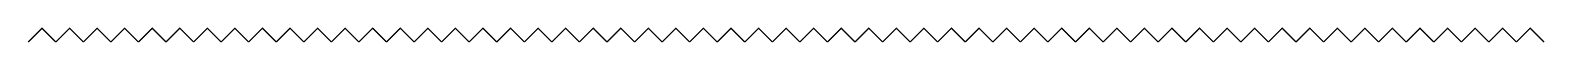
\begin{tikzpicture}[scale=0.35]
\foreach \x in {1,...,55}{
	\draw (\x,-0.25)--(\x+0.5,0.25)--(\x+1,-0.25);
}
\end{tikzpicture}
}

\usepackage{tikz}

\title{\textbf{ Examples:  Quadratic Reciprocity}}
\author{John D Mangual}
\date{}
\begin{document}

\fontfamily{qag}\selectfont \fontsize{25}{30}\selectfont

\maketitle

\noindent Analytic number theory is not my expertise.  Here we work out some softball examples related to quadratic reciprocity. \\ \\
Here's a question: \textbf{Can permutations be used to prove Artin reciprocity} or even parts of Class Field Theory? \\ \\
The proof of quadratic reciprocity seems like a random hodge-podge of techniques.\footnote{This is great for a first class when I was 15 years old it is not so great when you in graduate school are trying to learn Class Field Theory.} Can we unify some of these arguments using:
\begin{itemize}
\item Geometry of Numbers
\item Pigeonhole Principle
\end{itemize}
Gauss in his \textit{Disquiciones Arithmeticae} uses Pigeonhole to prove that $a^p \equiv 0 \mod p$. 

\newpage 

\noindent Any other applications? \\
\begin{tikzpicture}
\draw (0,0)--(19,0);
\end{tikzpicture} \\
Quadratic Reciprocity is stated in the number theory of textbook by \textbf{Hardy + Wright} in a Chapter called 
\begin{center} {\color{green!80!white}Fermat's Theorem and its Consequences}\end{center} \textit{after} his discussion of other more advanced topics
\begin{itemize}
\item prime numbers
\item Farey fractions
\item irrational numbers
\item congruences
\end{itemize}
I dislike prime number theory.  Papers in that subject are quite tedious to read.\\ 
\begin{tikzpicture}
\draw (0,0)--(19,0);
\end{tikzpicture} \\
\\
Fermat's little theorem says, e.g. $27| 3^{26}-1$:
$$ a^p = a \mod p$$
a theorem that I really like is that $5 = 2^2 + 1^2$:
$$ p = a^2 + b^2 \iff p = 4k+1 $$

\newpage

\newpage  

\noindent For proof of Quadratic Reciprocity I always refer to
\begin{itemize}
\item John Conway, \textbf{The Sensual Quadratic Form}
\end{itemize}
and he will use a proof by Zolotarev, involving the permutation group. \\ \\
So let's get started.

\newpage

\noindent The Legendre symbol is defined to be 
$$ \left(\frac{a}{p}\right) \equiv \left\{ 
\begin{array}{cc} 
1 & \text{ if }a \equiv x^2 \text{ mod } p \\
0 & \text{ if }a \not\equiv x^2 \text{ mod } p \\
\end{array}\right. $$
an indicator that $ x^2 = a \text{ mod }p$ has a solution.
$$ -1 \equiv 6\times 6  \text{ mod }37$$
So that $35$ is a perfect square mod $37$. 
$$ 5  \not \equiv x^2 \text{ mod }37$$ 
This is found by exhaustive search.  Therefore
$$ 5 \times (-1) \equiv 32 \not \equiv x^2 \text{ mod }37 $$
and maybe it is also a surprise that 
$$ 5 \times 6 \equiv 30  = 18 \times 18 \text{ mod }37$$
The complete list (sorted is):
{\normalsize
$$[0, 1, 1, 3, 3, 4, 4, 7, 7, 9, 9, 10, 10, 11, 11, 12, 12, 16, 16, 21, 21, 25, 25, 26, 26, 27, 27, 28, 28, 30, 30, 33, 33, 34, 34, 36, 36]
 $$}
\noindent here is how the numbers appeared in order.  
{\normalsize
 $$[0, 1, 4, 9, 16, 25, 36, 12, 27, 7, 26, 10, 33, 21, 11, 3, 34, 30, 28, 28, 30, 34, 3, 11, 21, 33, 10, 26, 7, 27, 12, 36, 25, 16, 9, 4, 1]$$}
The basic susprise is that a non-square times a non-square is again a square.  For example, $3 \times 7 = 21$ is not a square, so this is not true in $\mathbb{Z}$. \\ \\
This is our first taste of the weirdness of $\mathbb{Z}$. 

\newpage

\noindent A few surprises from information theory
\begin{itemize}
\item non-$\square$ must be found by exhaustive search
\item $\square$ stop as soon as we find one solution
\item non-squares $\times$ non-square $=$ square
\end{itemize}
Then there is another surprise that we can flip the number we're square-rooting and the modulus around.  There is \textbf{reciprocity}.\footnote{I am still not doing a great job of motivaing congruence arithmetic.  Sure it's the stuff that encrypts your e-mail and keeps your bank info secure.  But really why do you care?  \\ \\
Any time we talk about a \textbf{pattern} we resort to the language of periodicity and to integers.  And any time we talk about frequency -- how often something happens.  I will take my bus/car/bicycle/walk to work and I will go back home.  And these two things will happen once each day.  \textit{usually}} \\ \\
If we have two prime numbers, we can compare the possibility these are perfect square:
\begin{eqnarray*}
x^2 \equiv p \text{ mod }q \\
y^2 \equiv q \text{ mod }p \\
\end{eqnarray*}
and the outcomes depend on the parity.  Sometimes
\begin{itemize}
\item $x \text{ is }\square\leftrightarrow y\text{ is }\square$
\item $x \text{ is }\square \leftrightarrow y\text{ is not }\square$
\end{itemize}
\newpage 


\noindent The odds of $x$ being a perfect square is 50/50 in congruence arithmetic and we are asking for the overlap of two events occuring 50/50 chance. \\ \\
I would guess $(\frac{p}{q}) = 1$ about half the time and   $(\frac{q}{p}) = 1$ so maybe about half the time they should match up and half the time not.\footnote{I am just totally making this stuff up.  This is not mathematics, just a bunch of equations I'm writing on the board.}

\newpage

\noindent The Legendre symbol is defined to be 
$$ \left(\frac{a}{p}\right) \equiv \left\{ 
\begin{array}{cc} 
1 & \text{ if }a \equiv x^2 \text{ mod } p \\
0 & \text{ if }a \not\equiv x^2 \text{ mod } p \\
\end{array}\right. $$
and the theorem of quadratic reciprocity is that
$$ \left(\frac{p}{q}\right)\left(\frac{q}{p}\right)
= (-1)^{\frac{p-1}{2} \cdot \frac{q-1}{2}} $$
John Conway feels that proving this result with permutations leads to a simple argument.   Makes no use of the notion of a 
\begin{itemize}
\item prime number or
\item perfect square number.
\end{itemize}
He defines permutations like $\times a \text{ mod n}$
$$ \times 3 \text{ mod }11 = (0)(1,3,9,5,4)(2,6,7,10,8) $$
{\color{red!20!white}this is an even permutation}\\
this has an \textbf{even number} of {\color{green!80!white}cycles of even length}.  \\ \\
So this is a very particular character of the permutation group that he defines.  And he may have very good reasons for that. \\ \\
I still have to show that Zolotarev's definition on the cycles of the orbits of $\times a$ are the same as deciding if $x^2 \equiv a$ has a solution.\\\\
\begin{tikzpicture}
\node (a) at (0,0) {0};

\node (b) at (2,0) {1};
\node (c) at (4,0) {3};
\node (d) at (6,0) {9};
\node (e) at (6,2) {5};
\node (f) at (4,2) {4};

\node (g) at (8,0) {2};
\node (h) at (10,0) {6};
\node (i) at (12,0) {7};
\node (j) at (12,2) {10};
\node (k) at (10,2) {8};


\draw[->] (b)--(c)--(d)--(e)--(f)--(b);
\draw (g)--(h)--(i)--(j)--(k)--(g);
\end{tikzpicture} \\
There is a fair bit of sleight of hand in Conway's proof (as usual)
\newpage

\noindent 

\fontfamily{qag}\selectfont \fontsize{12}{10}\selectfont


\begin{thebibliography}{}

\item Jared Weinstein. \textbf{Reciprocity laws and Galois representations: recent breakthroughs} Bull. Amer. Math. Soc. 53 (2016), 1-39 

\item David A Cox. \textbf{Primes of the Form $x^2+ny^2$: Fermat, Class Field Theory, and Complex Multiplication} Wiley, 2013.

\item \textbf{A prime ideal $\mathfrak{p}$ decomposes in $\mathbb{Q}(\zeta_{24})/\mathbb{Q}(\sqrt{-6})$ iff it is generated by $\alpha\in1+2\Bbb{Z}[\sqrt{-6}]$} \\ \texttt{http://mathoverflow.net/q/234570/1358}

\item Roy L. Adler \textbf{Symbolic dynamics and Markov partitions}  Bull. Amer. Math. Soc. 35 (1998), 1-56  \\ \texttt{http://www.ams.org/journals/bull/1998-35-01/S0273-0979-98-00737-X/}


\end{thebibliography}



\end{document}